\chapter{Creation of Framework}
%Create a flowchart explaining the steps in the framework
%Explain each section in detail
%Explain creation of retrieving the input files using FAST API and OpenShift
%Explain storing of the framework in GitHub
%In this chapter, we will discuss the creation of the framework, steps involved and the implementation of it.
\section{Introduction}
\subsection{What is a Framework?}
A framework is a pre-built structure that provides a foundation for developing applications. It includes libraries, tools, and best practices that accelerate 
the development process. Frameworks serve as templates that can be customized to meet project requirements. Framework allow developers to work on the core, i.e,
the application of logic, rather than worrying about the underlying structure. Many frameworks are open-source and are easily available. Developers can also
contribute to the framework by adding new features or fixing bugs.

It is crucial to first understand your project requirements and determine which programming language and corresponding framework best suit those needs. 
Each framework is designed for a specific purpose and offers unique features. Having a fundamental understanding of the chosen programming language is 
essential for effectively working with the framework. Popular frameworks used today include Django, Flask, Angular, React, PyTorch, TensorFlow, and more. 
These frameworks empower developers to create robust and feature-rich applications.

\subsection{Why is a Framework used?}
Developing code from scratch can be a tedious and error-prone task. Clean, well-tested, and bug-free code is essential, but achieving this can be challenging.
Additionally, developers must adhere to coding standards and best practices to ensure code quality. Therefore, using frameworks that meet your requirements is
a better choice. Frameworks simplify the development process, reduce errors and provide a general template that can be customized as needed. They also make it
easier for others to understand your code, as they are likely familiar with the frameworks used. Frameworks offer several advantages, including:
\begin{itemize}
    \item Simplified testing and debugging of code.
    \item Clean and understandable code.
    \item Reduced code redundancy within the project.
    \item Decreased project time and cost.
    \item Modifiable and extendable features and functionalities provided by the framework.
\end{itemize}

\subsection{Libraries vs Frameworks}It is a common misconception that libraries and frameworks are the same. But they serve different purposes and have distinct characteristics. \newline \newline
\textbf{Libraries}:
\begin{itemize}
    \item A library is a collection of pre-written code that developers can use to optimize tasks.
    \item It provides specific functionality that can be called upon when needed.
    \item Developers have control over the flow of the application and decide when to use the library.
    \item Some of the popular libraries include NumPy, Pandas, Matplotlib, and more.\newline
\end{itemize}


\textbf{Frameworks}:
\begin{itemize}
    \item A framework is a pre-built structure that provides a foundation for developing applications.
    \item It dictates the architecture and flow of the application.
    \item Developers must adhere to the structure and guidelines set by the framework.
    \item Examples of popular frameworks include Django, Flask, Angular, React, and more. \newline
\end{itemize}

\section{Overview of the Framework}

Before, building a framework, it is essential to understand the requirements and objectives of the project. The main objective of this framework is to 
automate the process of running parametric simulations in Optislang, standardize and to verify the output files generated. The framework should be user-friendly,
easy to use, and provide detailed error logs in case of any issues.

After understanding the requirements, the next step is to design the framework. The framework should be designed in such a way that it is scalable,
modular, and easy to maintain. It should also be flexible enough to accommodate future changes and updates. 

This framework is built by with the help of classes, functions and libraries like \verb|Pandas|,\verb|NumPy| and other built in modules in Python.
Figure \ref{flowchart} shows a brief overview and working of the framework.
\newpage
%#Creation of flowchart using tikz
\begin{figure}[!ht]
    \centering
      \usetikzlibrary{shapes.geometric, arrows}
      \tikzstyle{box} = [rectangle, rounded corners, minimum width=3cm, minimum height=1.5cm, text centered, text width = 5cm, draw=black, fill=gray!8]
      \tikzstyle{io} = [trapezium, trapezium left angle=70, trapezium right angle=110, minimum width=3cm, minimum height=1cm, text centered, draw=black, fill=blue!30]
      \tikzstyle{image} = [minimum width=3cm, minimum height=1cm, text centered, text width = 2cm]
      \tikzstyle{process} = [rectangle, minimum width=3cm, minimum height=1cm, text centered, draw=black, fill=orange!30]
      \tikzstyle{decision} = [diamond, minimum width=3cm, minimum height=1cm, text centered, draw=black, fill=red!90, text = white]
      \tikzstyle{arrow} = [thick,->,>=stealth]
      \vspace{2cm}
    \begin{tikzpicture}[node distance=2.5cm]
        \node (clone_module) [image] {\centering 
\includegraphics[width=2cm]{Logo/github-mark.pdf}\newline Clone module};
        \node (check_json_files) [decision, below of = clone_module, yshift = -1.5cm] {\textbf{Check JSON Files}};
        \node (yes) [process, right of = check_json_files, xshift = 3cm] {\textbf{Yes}};
        \node (no) [process, left of = check_json_files, xshift = -3cm] {\textbf{No}};
        \node (create_parameters) [box, below of = yes] {\textbf{Create Parameters}};
        \node (get_input_files) [box, below of = create_parameters] {\textbf{Get Input Files}};
        \node (parametric_system) [box, below of = get_input_files] {\textbf{Create and run Parametric System}};
        \node (verify) [box, below of = parametric_system] {\textbf{Verify Output files}};
        \node (error_log) [box, below of = no] {\textbf{Display error : JSON files not found}};

        \draw [arrow] (clone_module) -- (check_json_files);
        \draw [arrow] (check_json_files) -- (yes);
        \draw [arrow] (yes) -- (create_parameters);
        \draw [arrow] (create_parameters) -- (get_input_files);
        \draw [arrow] (get_input_files) -- (parametric_system);
        \draw [arrow] (parametric_system) -- (verify);

        \draw [arrow] (check_json_files) -- (no);
        \draw [arrow] (no) -- (error_log);

    \end{tikzpicture}
    \caption{Flowchart of the framework}
    \label{flowchart}
\end{figure}


Let us understand the working of the framework in detail. The framework is mainly built using Python and uses Optislang's Python API to create and run the 
parametric simulations. The primary requirement for the framework to run is to have module present. Therefore, the first step is to clone the required module
from the specific repository and branch from GitHub. These serve us as the main arguments needed to run the framework. After cloning, the framework checks for 
\texttt{module\_config.json} and \texttt{parameters.json} files. These \acrshort{json} files are crucial to be present in the module as they contain the 
information required to run the parametric simulations automatically. The \texttt{module\_config.json} file contains information of 
the module like description of the module, name of the main script containing the algorithm, type of framework, input and output files and their properties.These data are important 
to create, run and verify the parametric system generated. The \texttt{parameters.json} file contains information about the parameters required to be set as input 
in the parametric system.
%# Display module_config.json and parameters.json?? Because it is very big and takes 1 and half page. Can also include it in Appendix...

At this stage, a decision is implemented. If the \acrshort{json} files are present, the framework proceeds to further steps. If the \acrshort{json} files are not found, the framework
comes to a halt and displays an error message being shown to the user. Figure \ref{error_message} shows the implemetation of the error message. This function is present
inside the class \texttt{ParametricSystem}.
\begin{figure}[!ht]
    \centering
    \renewcommand{\lstlistingname}{Code}
    \lstset{style=pythoncode}
    \begin{lstlisting}[language=python, caption= Function to verify existance of \acrshort{json} files, label={error_message}]
def json_files_log(self):
    try:
        if not self.get_module_config_path().exists():
            raise FileNotFoundError(
                f"{self.get_module_config_path()} does not exist"
            )
    except FileNotFoundError as e:
        print(
            f"{e} \nPlease ensure {self.get_module_config_path()} exists and re-run"
        )
    except Exception as e:
        print(e)
    try:
        if not self.get_parameters_path().exists():
            raise FileNotFoundError(f"{self.get_parameters_path()} does not exist")
    except FileNotFoundError as e:
        print(f"{e} \nPlease ensure {self.get_parameters_path} exists and re-run")
    except Exception as e:
        print(e)
\end{lstlisting}
\end{figure}



If the framework identifies the \acrshort{json} files, it process to the next step to create
parameters which are required to run the parametric system. These parameters are created based on the information present in the \texttt{parameters.json} file. These
parameters are then fed as input the parametric system during runtime.

The next step is to provide input files which are required by the parametric system in order to execute the simulations. These input files are being stored
in a pod in OpenShift. To retrieve these input files from OpenShift, an \acrshort{api} is setup using FastAPI. A detailed explanation of retrieving input files
from OpenShift is provided in Section \ref{}.

After the input files are retrieved, the framework then needs to create the parametric system. This should be achieved without the user's intervention, i.e, 
automatically. At this stage, we will be using the Python interpreter provided by Optislang as it includes the necessary libraries and functions to create and run 
the parametric system. Another terminal pops up which displays the progress of the execution of the system.

Since the whole process in the framework is automated, we need to ensure that the files generated by the parametric system are correct and are produced as 
expected. This is done by the function \texttt{verify\_output\_files} present in the class \texttt{ParametricSystem}. 


\section{Directory Structure} \label{directory_structure_section}
Before discussing the implementation of the framework, let us first understand how the files are structured within the framework. The directory structure is 
depicted in Figure \ref{directory_structure}. The framework consists of the following files and directories:
\begin{itemize}
    \item \textbf{\texttt{moo\_framework\_workflow.yaml}}:\newline
    This file contains the workflow for running the framework automatically. It is written in \acrshort{yaml} and is later used inside GitHub Actions.
    %! Add the reference to the section where the workflow is explained
    \item \textbf{\texttt{src}}:\newline
    This directory contains the source code of the framework. It consists of files which are used to create and run the parametric system in Optislang. It also
    consists of some helper functions which are used to build complex functions and classes for the creation of framework. We will discuss more about these files
    in section %! Add the reference to the section where the files are explained
    .
    \item \textbf{\texttt{tests}}:\newline
    This directory contains test cases for the framework. Section %! Add the reference to the section where the tests are explained
    explains the test cases in detail.
    \item \textbf{\texttt{main.py}}:\newline
    This python file calls the files which are responsible for the framework creation from  \texttt{src} directory . It is the main file for running the framework.
    \item \textbf{\texttt{requirements.txt}}:\newline
    This file contains the list of libraries which helps in running the framework. It is important to install these libraries before running the framework.
\end{itemize}
\newpage %#####
\begin{figure}[!ht]
  \centering
  \newcommand{\githubicon}{
\includegraphics[height=0.4cm]{Logo/github-mark.pdf}}
  \newcommand{\foldericon}{
\includegraphics[height=0.4cm]{Logo/folder_icon.pdf}}
  \newcommand{\pythonicon}{
\includegraphics[height=0.5cm]{Logo/python-logo-only.pdf}}
  \newcommand{\txticon}{
\includegraphics[height=0.5cm]{Logo/txt-svgrepo-com.pdf}}
  \newcommand{\ymlicon}{
\includegraphics[height=0.5cm]{Logo/GitHub Actions.pdf}}

  \begin{forest}
    for tree={
      font=\ttfamily,
      grow'=0,
      child anchor=west,
      parent anchor=south,
      anchor=west,
      calign=first,
      edge path={
        \noexpand\path [draw, \forestoption{edge}]
        (!u.south west) +(7.5pt,0) |- node[fill,inner sep=1.25pt] {} (.child anchor)\forestoption{edge label};
      },
      before typesetting nodes={
        if n=1
          {insert before={[,phantom]}}
          {}
      },
      fit=band,
      before computing xy={l=15pt},
    }
  [MOO Module Framework, label={right:\githubicon}
    [.github, label={right:\foldericon}
      [workflows, label={right:\foldericon}
        [moo\_framework\_workflow.yaml, label={right:\ymlicon}]
      ]
    ]
    [src
      [\_\_init\_\_.py, label={right:\pythonicon}]
      [create\_parametric\_system.py, label={right:\pythonicon}]
      [input\_files.py, label={right:\pythonicon}]
      [parametric\_system.py, label={right:\pythonicon}]
      [run\_parametric\_system.py, label={right:\pythonicon}]
      [utils.py, label={right:\pythonicon}]
    ]
    [tests
      [tests.py, label={right:\pythonicon}]
    ]
    [main.py, label={right:\pythonicon}]
    [requirements.txt, label={right:\txticon}]
  ]
  \end{forest} 
  \caption{Directory structure of the framework}
  \label{directory_structure}
\end{figure}

\section{Implementation of the Framework}
In this section, we will discuss the working and functioning of each of the files present in the framework.
\subsection{Source Code Overview}
The source code of the framework is present in the \texttt{src} directory. Figure \ref{directory_structure} shows the files present in the \texttt{src} directory.
Let us understand what each file contributes to the proper functioning of the framework.

\subsubsection{\textbf{\texttt{\_\_init\_\_.py :}}}
This is a special file in Python that is executed when a package is imported. It is used to define packages and can be used to initialize
their namespaces. Python would not recognize the directories as packages without this file.

Here, we have used this file to import the class \texttt{ParametricSystem} from the file \texttt{src/parametric\_system.py} which is later being called
inside \texttt{main.py}.
  
\renewcommand{\lstlistingname}{Code}
\lstset{style=pythoncode}
\begin{lstlisting}[language=python, caption={\texttt{\_\_init\_\_.py}}, label={init_file}]
from .parametric_system import ParametricSystem
\end{lstlisting}

\subsubsection{\textbf{\texttt{utils.py :}}}
This file is crucial as it serves as a backbone of the framework. This file contains functions that are used to build complex functions and classes which are
responsible for the proper implementation of the framework. 
\begin{figure}[!h]
  \centering
  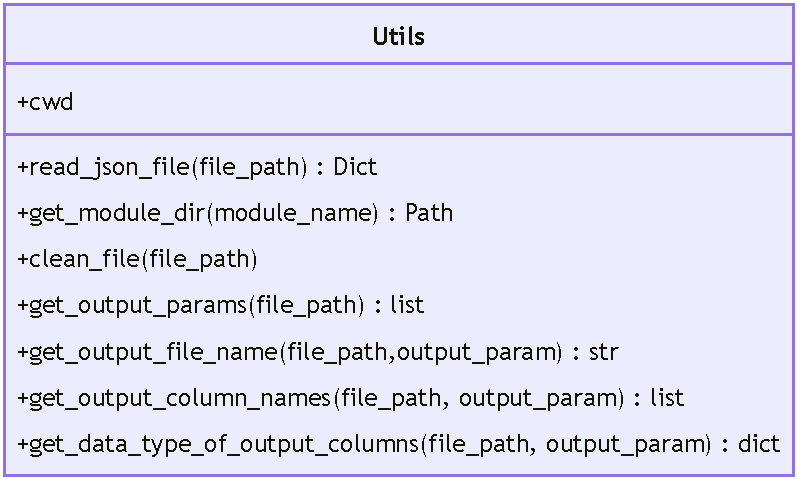
\includegraphics[width=0.6\textwidth]{Images/utils.pdf}
  \caption{Overview of functions in \texttt{utils.py}}
\end{figure}


\begin{itemize}
    \item The variable \texttt{cwd} stores the path of the current working directory by using the \texttt{os} module.  
    \item The function \texttt{read\_json\_file} reads the \acrshort{json} file and returns the data in the form of a dictionary. The function requires the 
    name of the \acrshort{json} file as an argument to get the data.
    \item \texttt{get\_module\_dir} function takes in the name of the module as an argument and returns the absolute path of the module directory.
    \item \texttt{clean\_file} function takes in the file path as an argument. This function is responsible for cleaning the file by removing the file.
    \item The function \texttt{get\_output\_params} takes in the path of \texttt{module\_config.json} file as an input and returns the list of output parameters
    defined in the \acrshort{json} file.
    \item \texttt{get\_output\_file\_name} function returns the name of the output file based on the output parameter and the file path of \texttt{module\_config.json} 
    provided in the argument.
    \item \texttt{get\_output\_column\_names} function takes in \texttt{module\_config.json}'s file path and the output parameter as input and returns a list 
    of column names present in the output file.
    \item \texttt{get\_data\_type\_of\_output\_columns} function is used to get the data type of the columns present in the output file. This function takes in
    the file path of \texttt{module\_config.json} and the output parameter as input and returns a dictionary containing the data type of columns. 
  \end{itemize}

  The functions \texttt{get\_output\_params}, \texttt{get\_output\_file\_name}, \texttt{get\_output\_column\_names}, and \texttt{get\_data\_type\_of\_output\_columns}
  are mainly used in the last part of the framework where we verify the output files generated by the parametric simulations. Whereas, the functions 
  \texttt{read\_json\_file}, \texttt{get\_module\_dir}, and \texttt{clean\_file} are used in the core process of building the framework.

  %# Should I add code snippets here??

\subsubsection{\textbf{\texttt{create\_parametric\_system.py :}}}
This file is used to create and build a parametric system without the use of Optislang's \acrshort{gui}. This file is being ran in Optislang's Python interpreter
which has libraries and functions to create the system. Therefore, the file \texttt{create\_parametric\_system.py} and \texttt{run\_parametric\_system.py} 
are being ran outside the class \texttt{ParametricSystem}.
\begin{figure}[!ht]
  \centering
  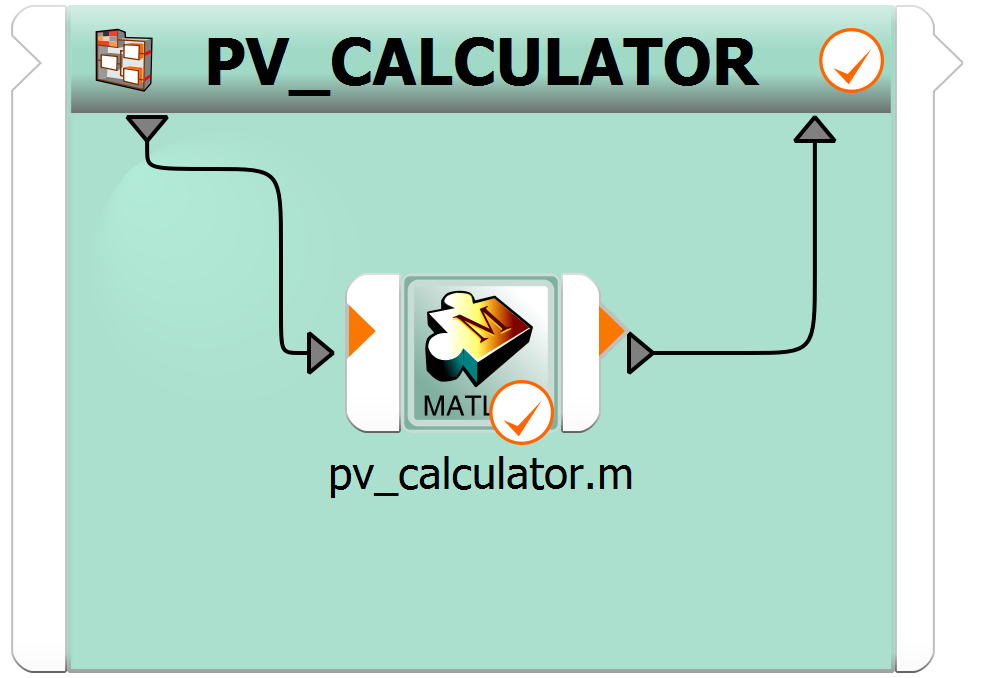
\includegraphics[width=0.4\textwidth]{Images/parametric_system_pv_calc.png}
  \caption{Example of a parametric system in Optislang}
  \label{parametric_system}
\end{figure}
 
Since, the whole creation process needs to be automated, the file \texttt{module\_config.json} helps us in creating the parametric system without the user's
intervention. The \acrshort{json} file contains key pair values which contain information like the name of the script containing the algorithm, type of framework 
which helps in creating the system. For example, in Figure \ref{parametric_system}, the system is getting the algorithm from the script \texttt{pv\_calculator.m}.
Type of framework refers to the type of module, Python or MATLAB. 

\renewcommand{\lstlistingname}{Code}
\begin{lstlisting}[style=pythoncode, caption= Function to create a parametric system, label={create_parametric_system}] ]
def create_parametric_actor(actor_name:str = get_module_name()):

    copy_file = actors.PythonActor('copy_input_files')
    parametric_system.add_actor(copy_file)

    if get_framework_type() == 'python':
        actor = actors.PythonActor(actor_name)
        parametric_system.add_actor(actor)
    elif get_framework_type() == 'matlab':
        actor = actors.MatlabActor(actor_name)
        parametric_system.add_actor(actor)

    #Connecting the python actor
    connect(parametric_system, 'IODesign', copy_file, 'IDesign')
    connect(copy_file, 'ODesign', actor, 'IDesign')
    connect(actor, 'ODesign', parametric_system, 'IIDesign')

    #Defining the path of the algorithm
    copy_file.path = str(Path(cwd,'src\\input_files.py'))
    if get_framework_type() == 'python':
        actor.path = str(path_to_algorithm())
    elif get_framework_type() == 'matlab':
        actor.file_path = str(path_to_algorithm())

    #Importing the parameters from the csv file
    params = parametric_system.parameter_manager
    params.import_from_csv(f'{cwd}\\optislang_actor_parameters.csv',',')
    parametric_system.parameter_manager = params

    #Reads the file 'optislang_parameters.py' which contains the necessary parameters for the actor to run
    exec(open(Path(cwd,'optislang_parameters.py')).read())
\end{lstlisting}
The function \texttt{create\_parametric\_actor()} takes in the argument actor name, which is the name of the actor to be displayed in the parametric system.
For the automation to function, we need to input the files required for the system to run automatically. The actor \texttt{copy\_file} is used to copy the input
files from OpenShift using Fast API. A detailed implementation of this is provided in section %#Provide section name for the explanation of retrieving input files from OpenShift.
Based on the type of module present, the actor \texttt{copy\_file} connects to either Python or MATLAB actor. This logic of connecting the actors depending on 
the module type is created as Optislang's Python API defines different functions to implement to create different actors. After connecting the actors, the path
for the actors is defined. The parameters are being created and fed to the system using the functions \texttt{generate\_optislang\_parameters\_from\_json()} and
\texttt{generate\_optislang\_parameters\_to\_csv()} which are present inside the class\texttt{ParametricSystem}. 
\begin{figure}[!ht]
  \centering
  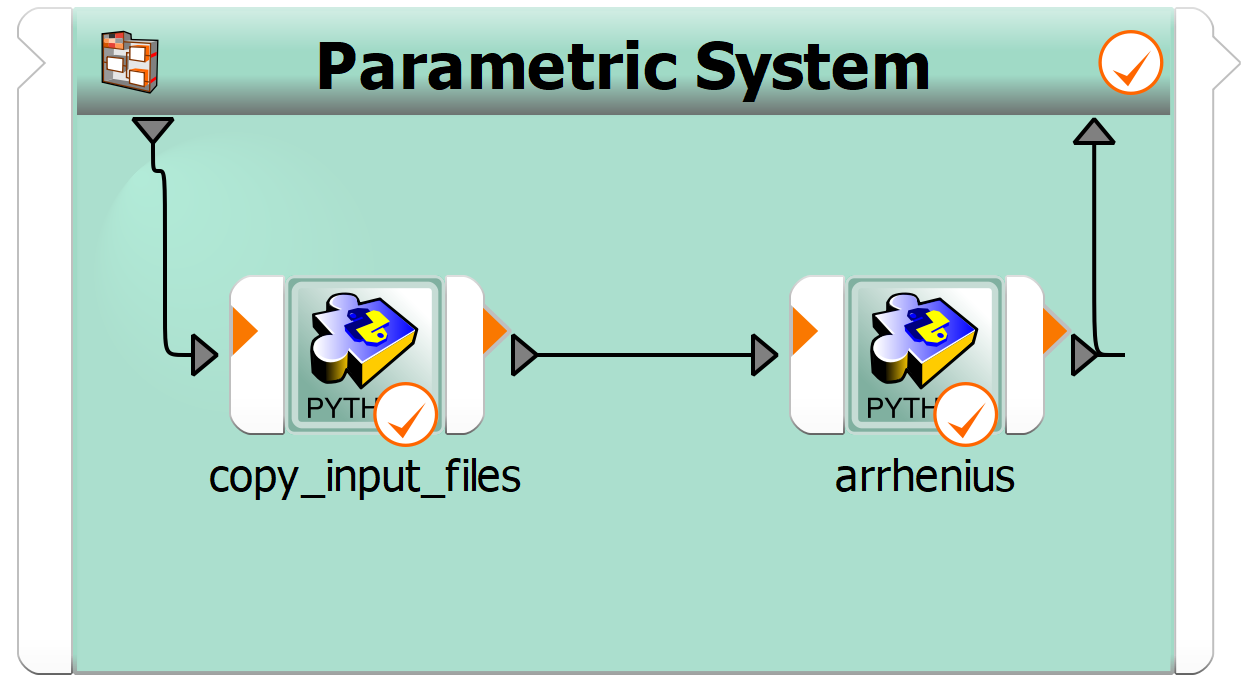
\includegraphics[width=0.5\textwidth]{Images/parametric_system_with_copy_actor.png}
  \caption{Example of a parametric system with copy actor}
  \label{parametric_system_with_copy_actor}
\end{figure}

\subsubsection{\textbf{\texttt{run\_parametric\_system.py :}}}
This file mainly calls the parametric system created in \texttt{create\_parametric\_system.py} and runs the system in Optislang's instance. This file is later
being called in the class \texttt{ParametricSystem} to run the parametric system. 
\renewcommand{\lstlistingname}{Code}
\begin{lstlisting}[style=pythoncode, caption={Overivew of \texttt{run\_parametric\_system.py}}, label={run_parametric_system}]
#Creating a parametric system
obj = actors.ParametricSystemActor("Parametric System")
obj.auto_save_mode = AS_ACTOR_FINISHED
add_actor(obj)

#Reads the file 'optislang_parameters.py' which contains the design connections for the module
parametric_system = obj
cwd_ = os.getcwd()
cwd = Path(cwd_).parents[1]
exec(open(Path(cwd,'src','create_parametric_system.py')).read())
obj = parametric_system
\end{lstlisting}

\subsubsection{\textbf{\texttt{parametric\_system.py :}}}
This is the most important script in the framework. This file contains the class \texttt{ParametricSystem} which is mainly responsible for the creation of the
framework. Due to the complexity of the framework, we use \texttt{utils.py} to build the functions and classes. 
\begin{figure}[!ht]
  \centering
  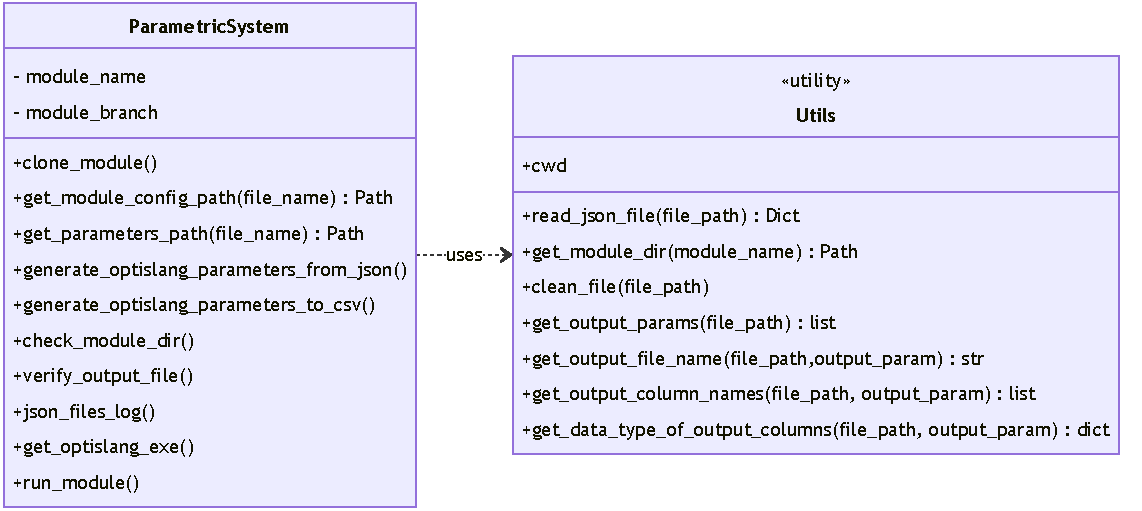
\includegraphics[width=0.9\textwidth]{Images/parametric_system_class.pdf}
  \caption{Overview of the class \texttt{ParametricSystem}}
  \label{parametric_system_class}
\end{figure}

Figure \ref{parametric_system_class} describes the methods used in the class \texttt{ParametricSystem}. The user needs to provide the name of the module and
the name of the branch from where the module needs to be cloned. The class \texttt{ParametricSystem} contains the following methods:  
\begin{itemize}
  \item \textbf{\texttt{clone\_module()}}:\newline
  This method is used to clone the module from the GitHub repository by using the arguments provided by the user. The function \texttt{clone\_module()} tries 
  to delete if an existing module is present and clones the module from the repository.

  \item \textbf{\texttt{get\_module\_config\_path()}}:\newline
  This function returns the path of \texttt{module\_config.json} file. This functions takes in name of the file as an argument and the returns the absolute path
  of the file.

  \item \textbf{\texttt{get\_parameters\_path()}}:\newline
  This functions acts similar to \texttt{get\_module\_config\_path()} but returns the path of \texttt{parameters.json} file. This function take sin the name of 
  the file as an argument and returns the absolute path of the file.
  
  \item \textbf{\texttt{generate\_optislang\_parameters\_to\_csv()}}:\newline
  To input the parameters inside the parametric system, the parameters are being fed in a \texttt{csv} format. To achieve this, the function \texttt{generate\_
  optislang\_parameters\_to\_csv()} is used. This function takes in the path of \texttt{parameters.json}, reads the data in it and converts it into a \texttt{csv}
  format. Later, this \texttt{csv} is saved in the current working directory as \texttt{optislang\_actor\_parameters.csv}.

  \item \textbf{\texttt{generate\_optislang\_parameters\_from\_json()}}:\newline
  Optislang requires the user to provide the parameters not only in \texttt{csv} format, but also while creating the system. To overcome this, this function
  creates the parameters from the data provided in \texttt{parameters.json}. Later, the data is being saved as \texttt{optislang\_parameters.py} containing the 
  parameters required. This is later being used inside \texttt{create\_parametric\_system.py} as shown in figure \ref{create_parametric_system}.

  \item \textbf{\texttt{check\_module\_dir()}}:\newline
  While creating the modules, the system developers have hardcoded the path of the module in many of their functions. To work around this, this function mocks
  the module directories by creating a new directory called \textbf{\texttt{Module}} containing the child directories, \texttt{02\_Model} and \texttt{04\_Input} 
  respectively. \texttt{02\_Model} contains the Optislang simulation file and its corresponding input and output files. Modules like \texttt{ARRHENIUS} and
  \texttt{COFFIN MANSON} needs a specific input file to be saved in \texttt{04\_Input}. If there is a previously existing folder named \texttt{Module}, it 
  ensures to remove the contents of it and create a new one. 

  \item \textbf{\texttt{verify\_output\_files()}}:\newline
  This function is primarily used to verify the existence and correctness of the output files generated by the parametric system. This function is used after
  the parametric system is created. Figure \ref{verify_output_files} shows a brief overview of the function. 
  \begin{figure}[!ht]
    \centering
    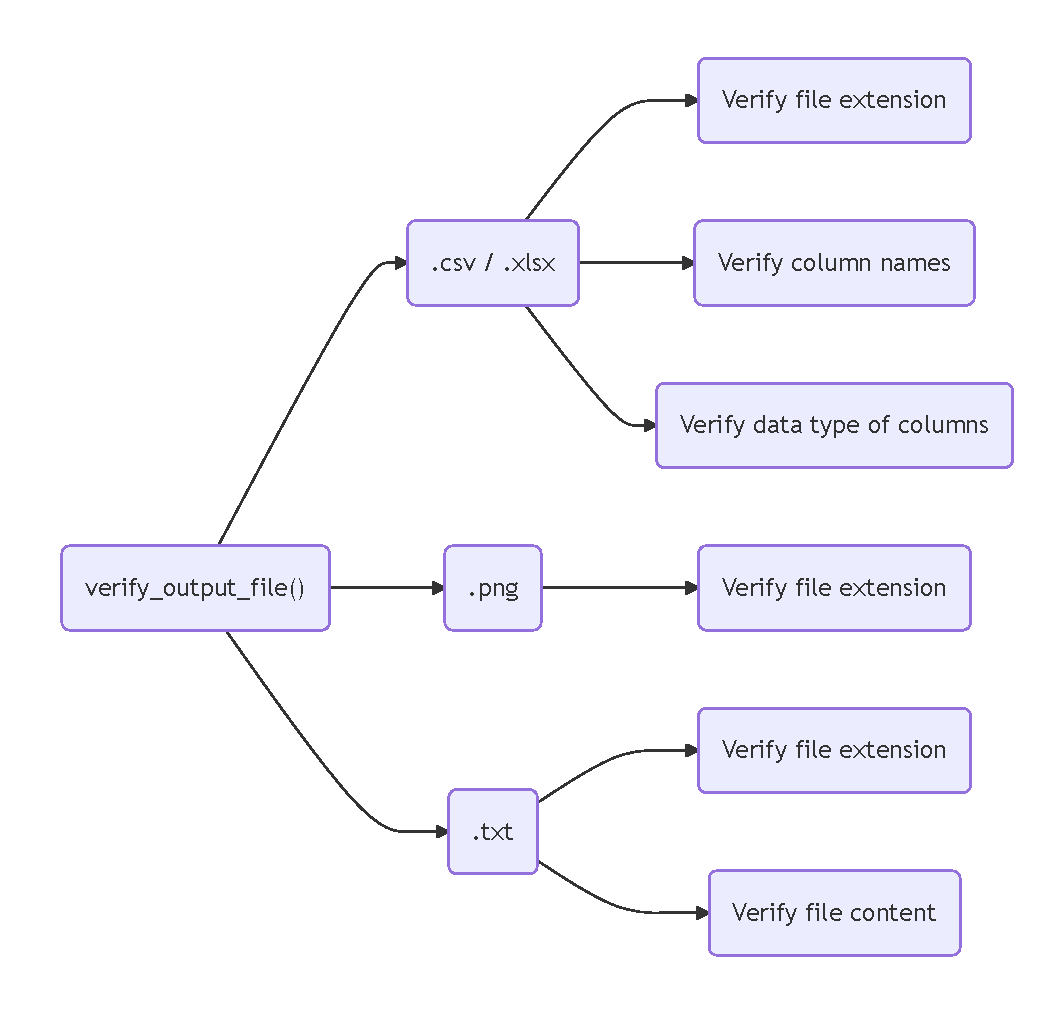
\includegraphics[width=0.8\textwidth]{Images/verify_output_file.pdf}
    \caption{Overview of \texttt{verify\_output\_files()} function}
    \label{verify_output_files}
  \end{figure}
  
  To verify the output, we first get the data to verify from the \texttt{module\_config.json}. This data contains the properties of output files like column 
  names, name of the output file, it's format and data type of the columns. The functions gets the folder containing the output files and iterates it through
  one by one to verify if all the output files are present. After verifying the existence of the output files, the algorithm checks if the columns present in
  the output files match the columns present in the \texttt{module\_config.json}.Here, it uses the library \texttt{Pandas} to read the \texttt{csv} files. 
  After verifying the columns, the algorithm continues to check for the data type of the columns. If all the checks are passed, it shows a success message 
  stating that the output files are correct. If any of the checks fail, it shows that the output files have an issue displaying the specific error message.

  Since all the outputs are not in a \texttt{csv} file, the function also needs to check for output files of type \texttt{.txt} and \texttt{.png}. To check
  for \texttt{.png}, we only just verify if the file is present and the file name is correct. For \texttt{.txt} files, we do the same by verifying the existence
  of the file and the file name. In addition to that, it also opens and verifies if the generated \texttt{.txt} file is empty or not.  

  \item \textbf{\texttt{json\_files\_log()}}:\newline
  This function provides us a detailed error message if any one of the \texttt{\acrshort{json}} files are not found. A detailed explanation of this function
  is already explained in Figure \ref{error_message}.

  \item \textbf{\texttt{get\_optislang\_exe()}}:\newline
  Since the framework is designed to run automatically, it is essential not to hardcode the path any of the files. This function's goal is to provide the location
  of Optislang's executable file. This is achieved by using \texttt{os.getenv()} function from the built-in module \texttt{os}, which returns the value of the environment variable containing the
  path of the Optislang executable file. If the path is not found, the function raises an error message.

  \item \textbf{\texttt{run\_module()}}:\newline
  This function calls the other functions present in an orchestrated manner as shown in figure \ref{flowchart} to run the module. In this function, initially, 
  it clears all the existing files and folders cerated during the previous run to avoid any conflicts. Later, it clones the module, checks for the \acrshort{json}
  files, creates the parameters, retrieves the input files, creates the parametric system and finally runs it.  

\end{itemize}

\section{Testing of Framework}
While building the framework, it is also essential to test the framework to ensure that it is working as expected. One way to do is to include breakpoints, add print 
statements, and debug the code. However, this method is not efficient when the codebase is huge. Therefore, another way is to write unit cases for the framework.

Unit testing is a software testing method that involves testing a small unit of code, typically a function or method. They are crucial part of the development 
process as they help in identifying bugs and errors early in the development cycle. Python has two frameworks for unit testing, \texttt{unittest} and 
\texttt{pytest}. I have implemented \texttt{unittest} for testing since it is part of the Python's standard library. Here, the unit tests can be found 
in the \texttt{tests} directory. The file \texttt{tests.py} contains the test cases for the framework. Unit tests generally should cover the following aspects:
\begin{itemize}
  \item \textbf{Unit tests}:\newline
  This is used to test the functionalities of each individual methods and functions.
  \item \textbf{Integration tests}:\newline
  These tests are implemented to verify if the integration to the files are working as expected.
  \item \textbf{Boundary tests}:\newline
  This ensures to check the edge cases of the functions. For example, if the provided input is an empty string, the function should return an error message.
  \item \textbf{Negative tests}:\newline
  To check if the function handles incorrect input properly, negative tests are implemented. An example for this would be to handle if the argument is of a 
  different data type than expected. 
\end{itemize}

Figure \ref{unittest} shows an example of a unit test implemented in Python to test the existence of \acrshort{json} files. 
\renewcommand{\lstlistingname}{Code}
\begin{lstlisting}[style=pythoncode, caption={Example of a unit test}, label={unittest}]
class TestParametricSystem(unittest.TestCase):
    def setUp(self) -> None:
        self.parametric_system = ParametricSystem('MOO_M_ARRHENIUS','MOO-1355_py_framework_poc')
        self.cwd = os.getcwd()

    def get_module_name(self):
        for file_name in os.listdir(self.cwd):
            if file_name.startswith('MOO'):
                return Path(self.cwd,file_name)
        return None

    def test_get_module_config_path(self):
        self.assertIsNotNone(self.get_module_name(), 'Module folder not found.')
        expected_path = (Path(self.get_module_name(),'01_Specification', 'module_config.json'))
        actual_path = self.parametric_system.get_module_config_path()
        self.assertEqual(expected_path, actual_path)  
\end{lstlisting}

Firstly, we create a class \texttt{TestParametricSystem} which inherits from \texttt{unittest.TestCase}. To avoid initialization of the same variables in each
test case, we take advantage of the \textbf{\texttt{setUp()}} method. Here, we create an object an initialize the arguments for the class \texttt{ParametricSystem}.
The functions in the unit tests needs to start with the prefix \texttt{test}. This convention is used to identify the function which the test cases. For example, 
in Figure \ref{unittest},the function \texttt{test\_get\_module\_config\_path} recognizes that it is a test case whereas the function \texttt{get\_module\_name}
is a helper function and not a test case. In this example the function \texttt{test\_get\_module\_config\_path} is responsible to check if the path of the folder
containing the \acrshort{json} file is correct. To ensure this, we use the function \texttt{assertEqual} which checks if the expected path is equal to the 
actual path. If the paths are equal, the test case passes, else it fails. \texttt{unittest} provides several other functions to test the code. 

\section{Execution of Framework}
%! Explain main.py, which is the main file to run the framework
To execute the framework, the user needs to run the file \texttt{main.py}. This file is the main file to run the framework. This script calls the functions
from the class \texttt{ParametricSystem} and runs the module. Figure \ref{main_script} shows the execution of the framework.
\renewcommand{\lstlistingname}{Code}
\begin{lstlisting}[style=pythoncode, caption={Execution of framework using \texttt{main.py}}, label={main_script}]
from src import ParametricSystem

module_name = "MOO_M_ARRHENIUS"
module_branch_name = 'MOO-1355_py_framework_poc'

def main():
    system = ParametricSystem(module_name, module_branch_name)
    system.clone_module()
    if (
        system.get_module_config_path().exists() & system.get_parameters_path().exists()
    ) == True:
        system.run_module()
        system.verify_output_file()

    else:
        system.json_files_log()

if __name__ == "__main__":
    main()
\end{lstlisting}

In code snippet \ref{main_script}, an example of cloning the module \texttt{MOO\_M\_ARRHENIUS} is shown. An instance of the class \texttt{ParametricSystem} 
is created with the arguments \texttt{module\_name} and \texttt{module\_branch\_name}. Then, the check for the \texttt{\acrshort{json}} files is done. 
The verifying of the files is done outside the function \texttt{run\_module()} as we do need to verify the existence of the files before running the module.
Once the existence of the files are verified, the module is being run and after the successful execution in Optislang, it displays the status of the output
files. 

%# Also, explain the requirements.txt file

\subsection*{}
The working of \texttt{input\_files.py} will be explained in section %!Provide section name for the explanation of retrieving input files from OpenShift
wherein a detailed explanation of retrieving input files from OpenShift using Fast API is provided.


\section{Retrieve input files for Framework}
\subsection{Introduction}
%# Explain the idea before using the Fast API and OpenShift
%# What were the disadvantages of the previous method
%# The following sections are the tools used to retrieve the input files.
\subsection{Docker}
%# Intro to Docker
%# Use of Docker
%# Creation of an image
\subsection{OpenShift}
%# Intro to OpenShift
%# Explain the creation of a pod
\subsection{Fast API}
%# What is API
%# Intro to Fast API
%# How to use Fast API

\subsection{Implementation}
%# Explain the implementation of retrieving input files using Fast API and OpenShift
%# mock_blob_storage
%# Pushing docker image to OpenShift
%# Running the Fast API in OpenShift
%# Retrieving the input files using API calls